\documentclass[border=1pt]{standalone}
\usepackage[dvipsnames]{xcolor}
\usepackage{tikz}                       % Graphen und kommutative Diagramme
\usetikzlibrary{patterns}               % Um schraffierte Formen in der tikzpicture-Umgebung zu zeichnen.


\begin{document}
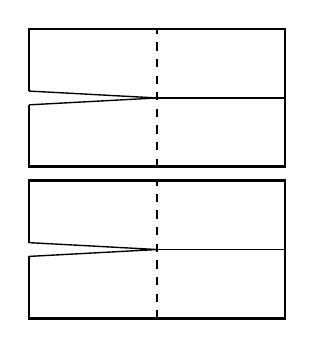
\begin{tikzpicture}[yscale=.7, xscale=1.3, x=1.25cm, y=1.25cm, line width=.5pt]
    \draw[color=black, line width=1pt] (0,0.9) -- (0,0) -- (2,0) -- (2,2) -- (0,2) -- (0,1.1);
    \draw[color=black] (0,0.9) -- (1,1) -- (0,1.1);
    \draw[color=black] (1,1) -- (2,1);
    \draw[color=black, dashed] (1,0) -- (1,2);
    
    \draw[color=black, line width=1pt] (0,3.1) -- (0,2.2) -- (2,2.2) -- (2,4.2) -- (0,4.2) -- (0,3.3);
    \draw[color=black] (0,3.1) -- (1,3.2) -- (0,3.3);
    \draw[color=black] (1,3.2) -- (2,3.2);
    \draw[color=black, dashed] (1,2.2) -- (1,4.2);
\end{tikzpicture}
\end{document}